\section{Experiment \& Result} \label{section:experiment_result}

\textbf{Oxford5K.} To prove our hypotheses, the authors test both the BoW systems with and without spatial rerank on the Oxford Building 5K Dataset \cite{oxbuilding}. This dataset was constructed by Philbin et al. in 2007 \cite{2}. It consists of 5,062 images of resolution $1024 \times 768$ belongs to 11 different Oxford buildings. Images for each building are collected from Flickr by searching using text queries. In figure \ref{fig:oxbuilding}, some samples from the dataset are shown. Along with the dataset, there are also 55 queries along with their ground-truth, 5 for each landmark, as shown in figure \ref{fig:oxbuilding_query}. The groundtruth of 55 queries are manually constructed. For each query, images are classified into 4 groups: (1) \textit{Good}: the building appears apparently, (2) \textit{OK}: more than 25\% of the building is present, (3) \textit{Bad}: the building is not shown up, and (4) \textit{Junk}: less than 25\% of the building is captured. The reason why the authors use this dataset is because of its popularity, it is used by many previous works in this field. Thus, we can easily compare our systems with those previous works.

\textbf{Evaluation protocol.} The performance of our system is evaluated by mean average precision (mAP). Since mAP is only described briefly in \ref{section:background_relatedworks}, we now give detailed formulas of mAP. If the set of relevant documents for q query $q_{j} \in Q$ is $\{d_{1}, ... d_{m}{j}\}$ and $R_{j}{k}$ is the set of ranked retrieval results from the top result until you get to document $d_{k}$, mAP(Q), Q is the set of queries, is defined as follow:

\begin{equation}
mAP(Q) = \frac{1}{|Q|}\times\sum_{j=1}^{|Q|} \frac{1}{m_{j}}\times\sum_{k=1}^{m_{j}}Precision(R_{j_{k}})
\end{equation}

To ensure the objectivity of evaluation process, the authors decide to use the already implemented C++ code to calculating mAP of the ranklist available at \cite{oxbuilding}. In this implementation, since AP approximates the area under the precision-recall curve of a query, mAP is therefore computed as the average area under precision-recall curves of all queries. Additionally, the set of relevant images for a query is defined as those images which are categorized as \textit{Good} or \textit{OK} in the corresponding groundtruth.

\begin{figure}
    \centering
    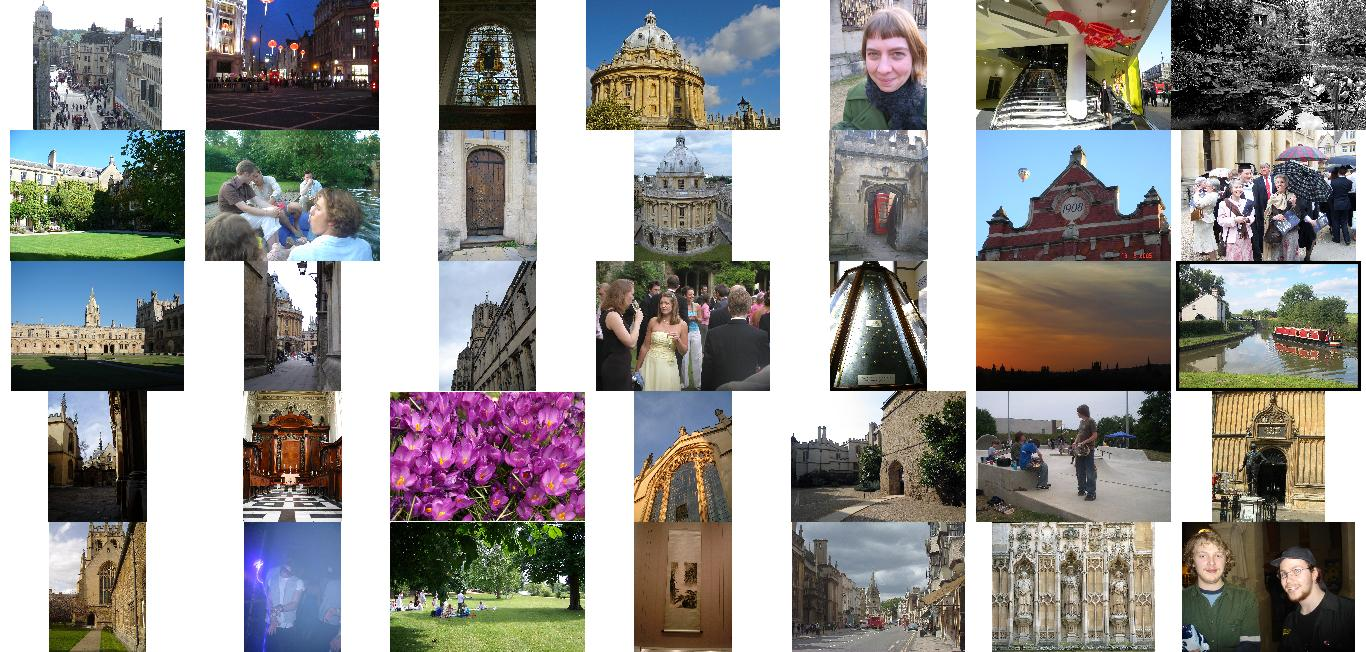
\includegraphics[width=3.0in]{oxbuilding.jpg}
    \caption{Some random images from Oxford Building 5K Dataset}
    \label{fig:oxbuilding}
\end{figure}

\begin{figure}
    \centering
    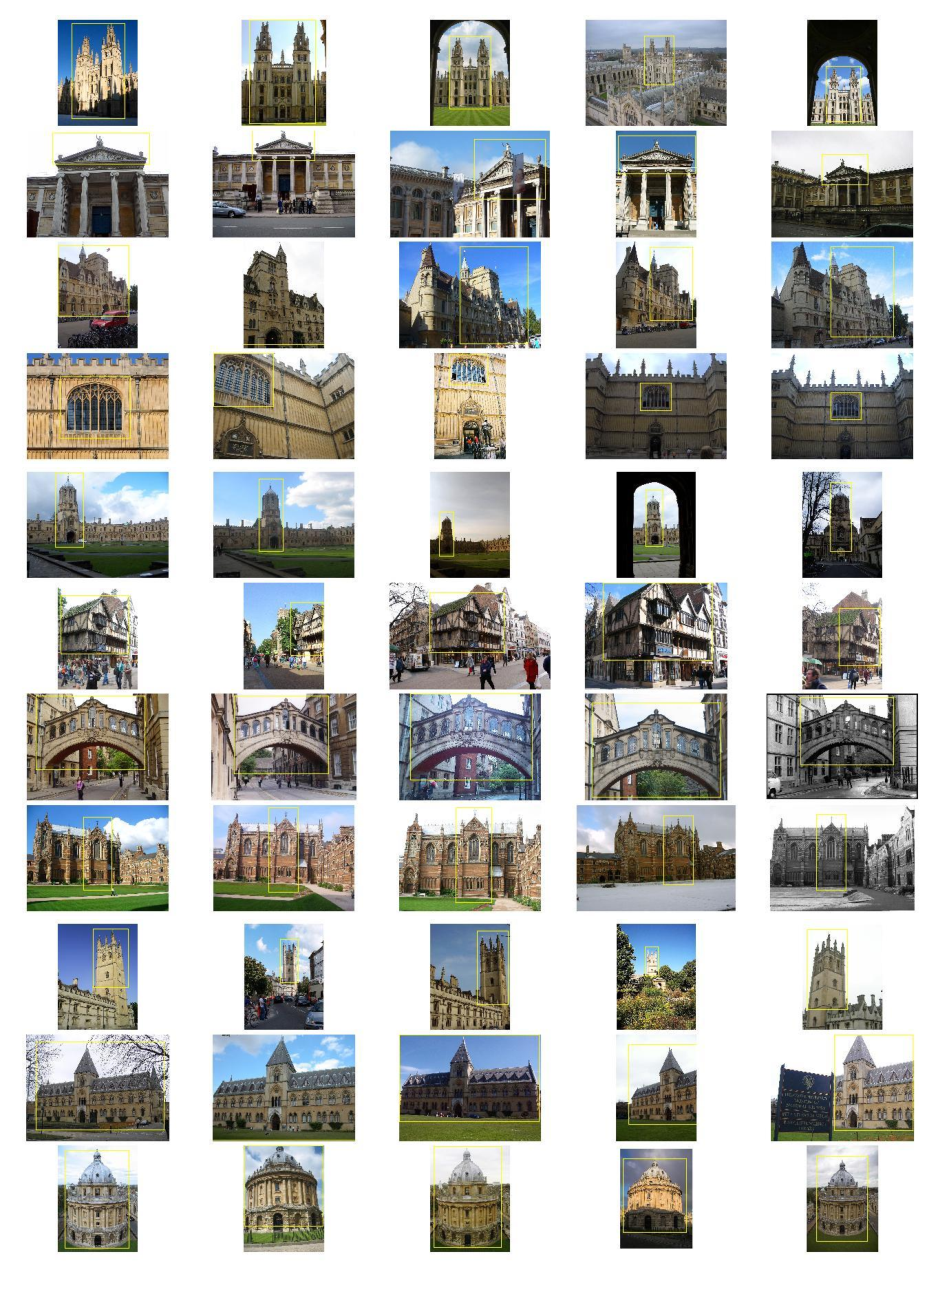
\includegraphics[width=3.0in]{oxbuilding_query.pdf}
    \caption{55 queries of Oxford Building 5K Dataset}
    \label{fig:oxbuilding_query}
\end{figure}

Our experiment shows that spatial rerank has significant impact on the retrieval quality of BoW model, an increase from 0.676 to 0.741 in term of mAP. The original BoW model have AP at least or higher than 0.5 for 41/55 queries and by using spatial rerank the figure is improved to 47/55 queries. Among 55 queries, there are 40 queries that achieve higher AP after incorporating spatial information and there 22 queries increasing more than 0.050. The highest boost is 0.583, from 0.417 to 1.000. However, there 2/55 queries suffering significant performance drop (decreases more than 0.100). To explain why there are performance reduction in these 2 queries, shown in figure \ref{fig:bad_queries}, the authors believe that they are affected by the background features which actually should not be considered in the rerank step. For better illustration, the APs of all 55 queries are given in \ref{fig:ap_chart}.

\begin{figure}
  
		\begin{subfigure}{.5\textwidth}
		\centering
    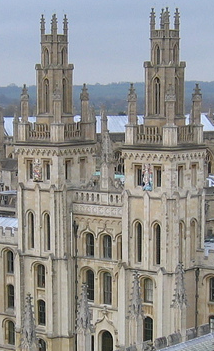
\includegraphics[width=3.0in]{all_souls_4_query.png}
		\end{subfigure}
		
		\begin{subfigure}{.5\textwidth}
		\centering
		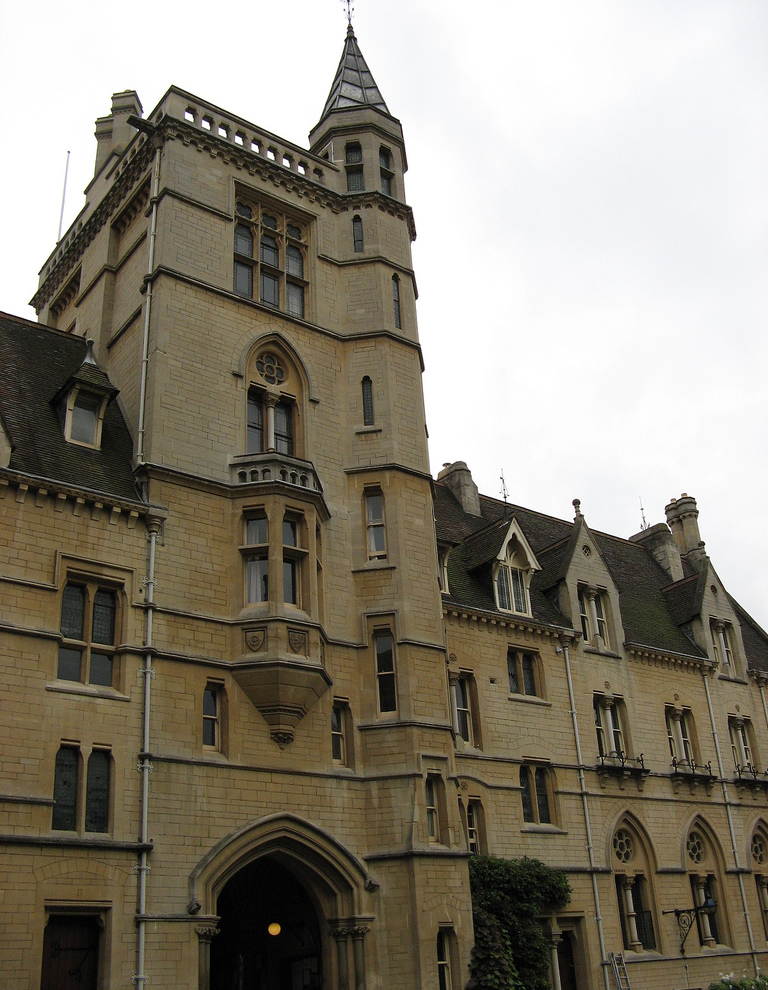
\includegraphics[width=3.0in]{balliol_2_query.png}
		\end{subfigure}
		
    \caption{Two queries having worse performance after using spatial rerank}
    \label{fig:bad_queries}
\end{figure}

\begin{figure}
  
		\begin{subfigure}{.5\textwidth}
		\centering
    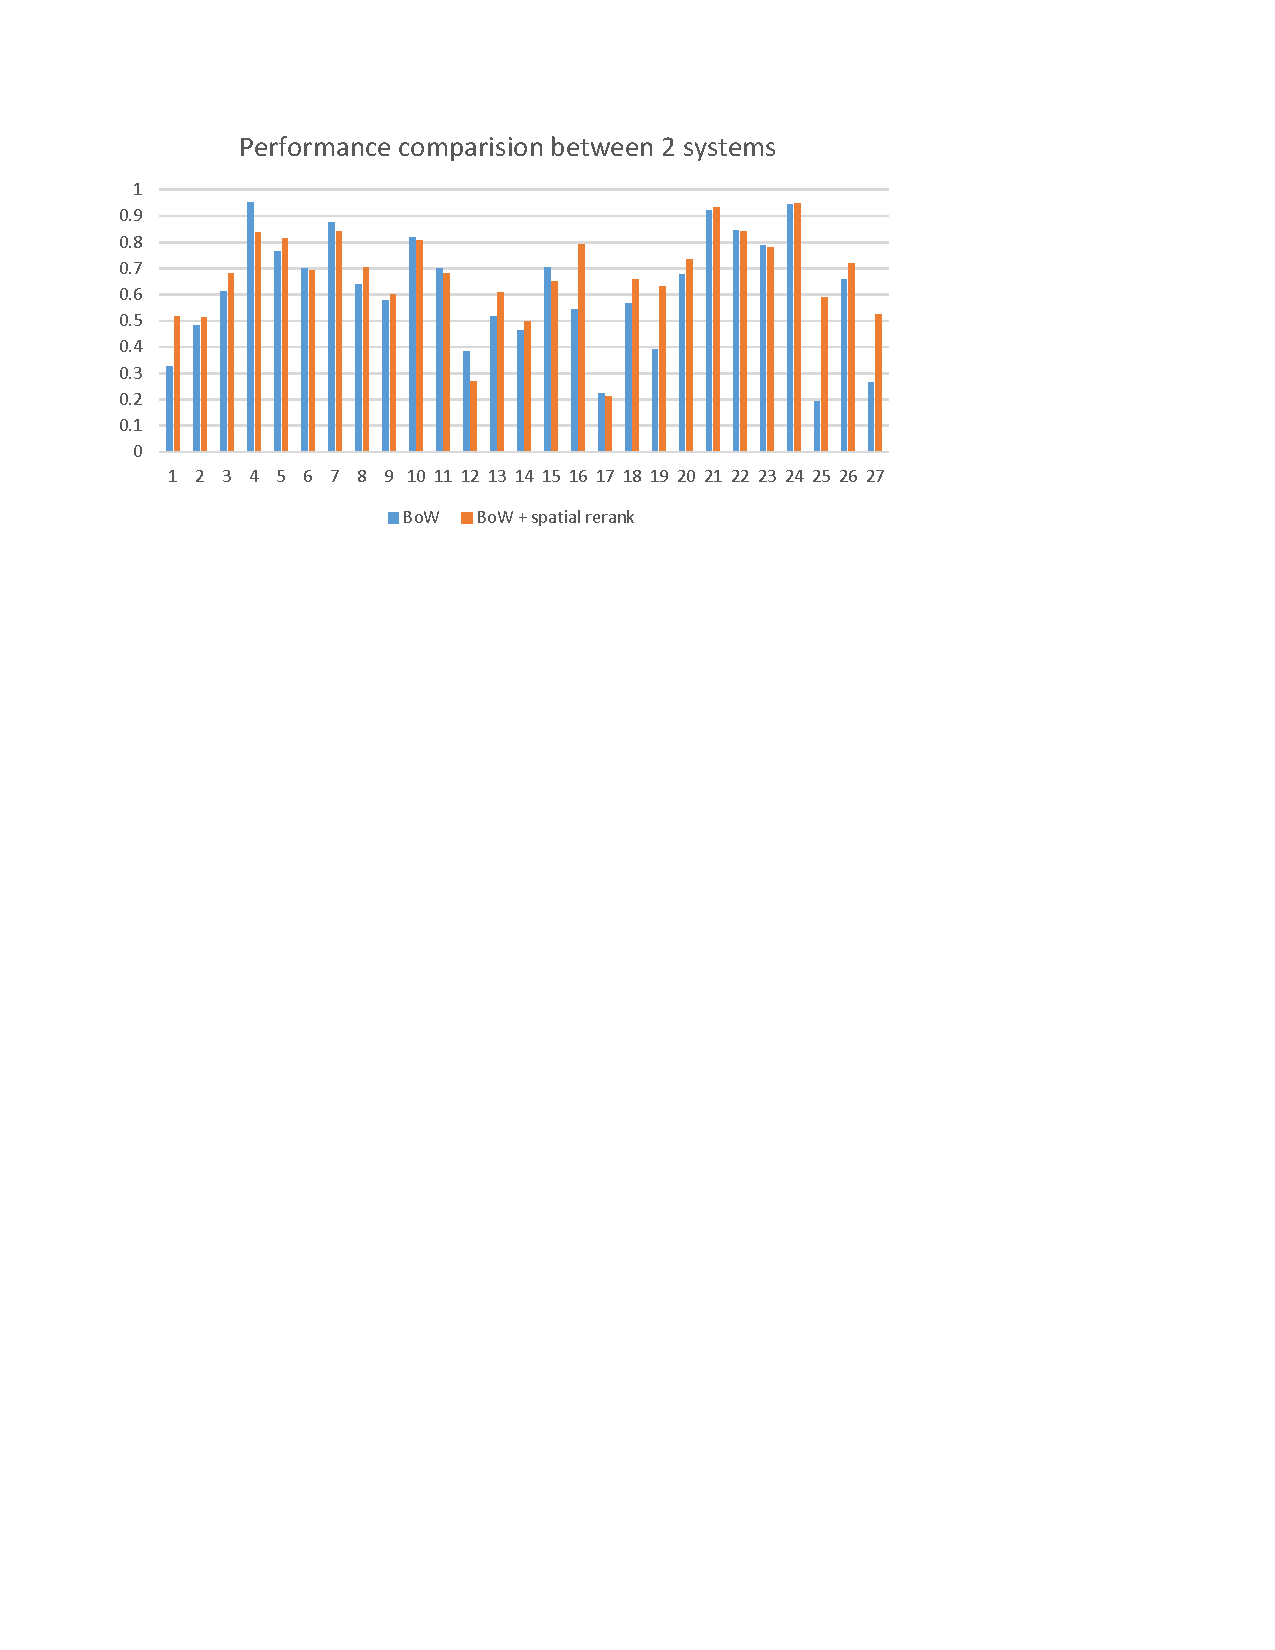
\includegraphics[width=3.0in]{ap1.pdf}
		\caption{APs of queries 1 - 27}
		\end{subfigure}
		
		\begin{subfigure}{.5\textwidth}
		\centering
		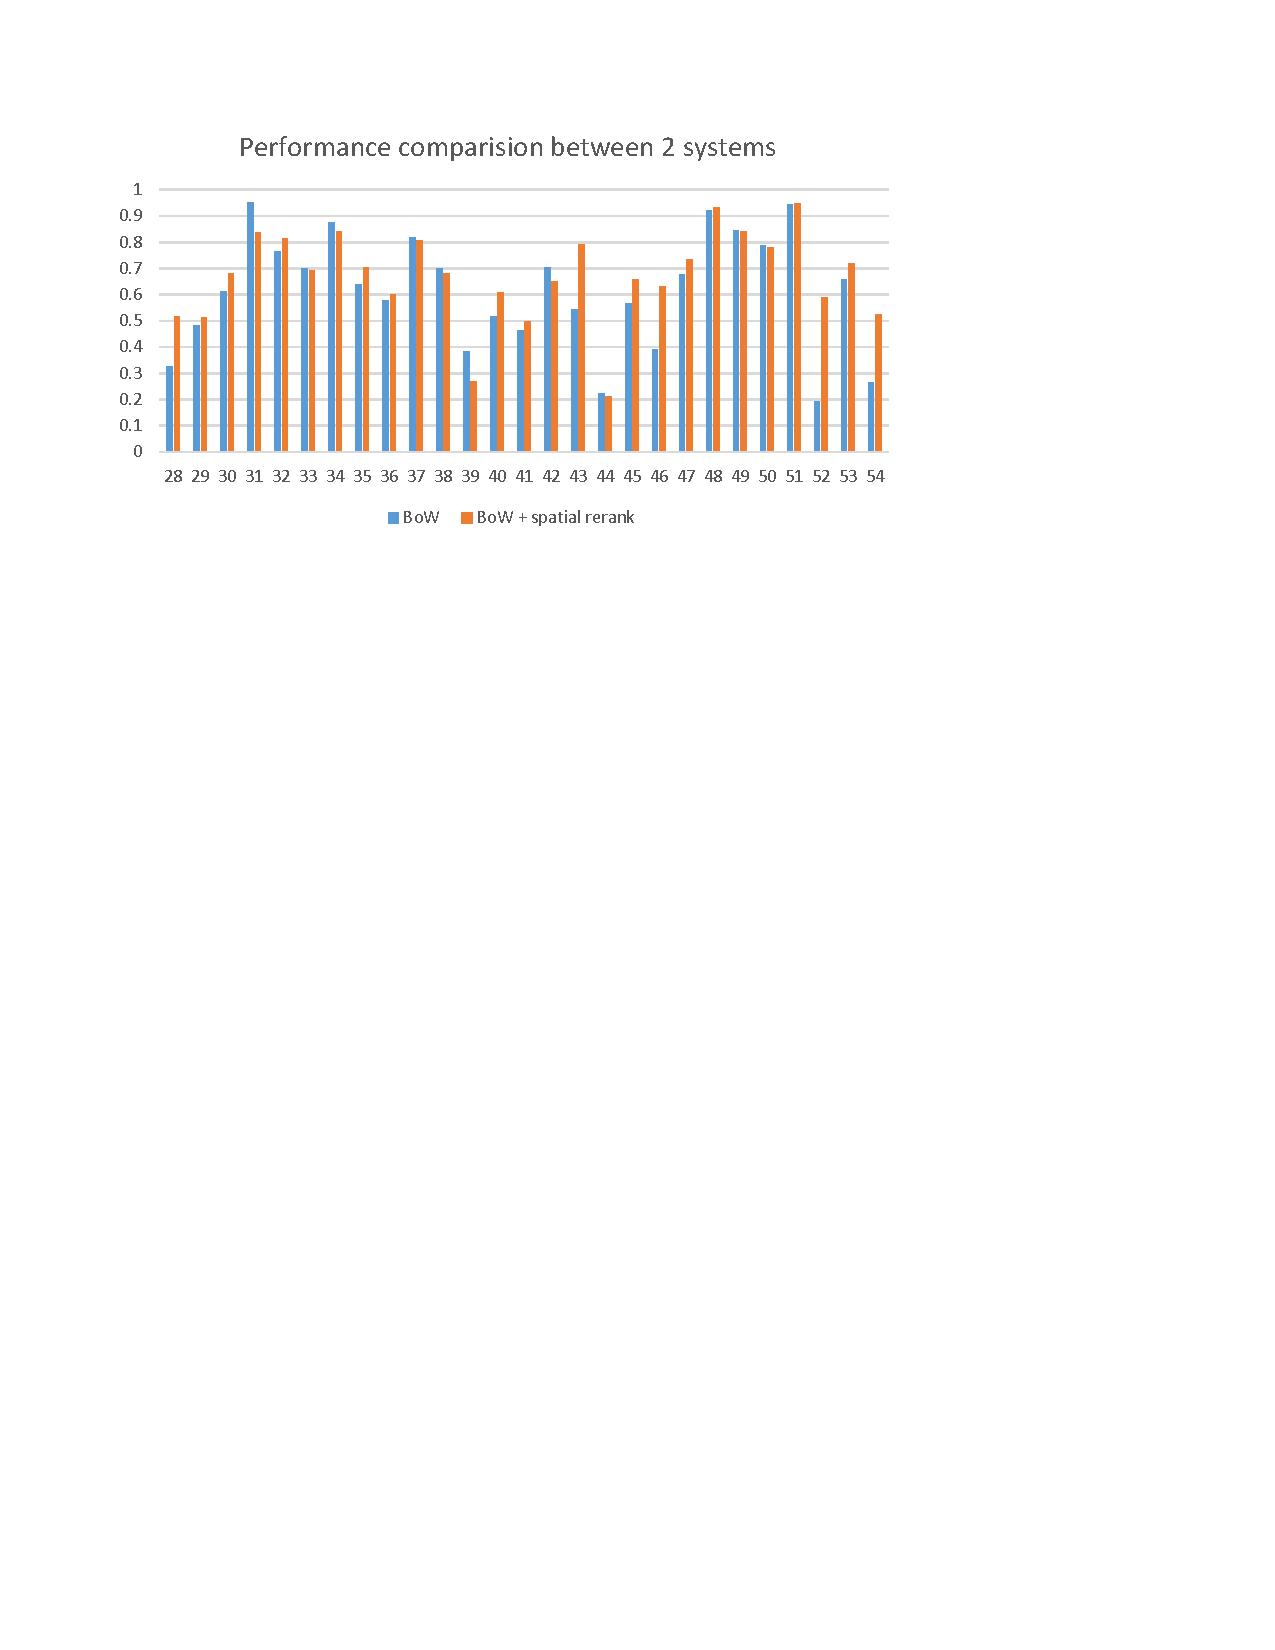
\includegraphics[width=3.0in]{ap2.pdf}
		\caption{APs of queries 28 - 55}
		\end{subfigure}
		
    \caption{Comparison chart between the 2 methods}
    \label{fig:ap_chart}
\end{figure}
